%cmd: clear; latex gull.tex
%cmd: clear; xdvi gull.dvi



\documentclass[a4paper,12pt]{article}

\usepackage[english]{babel}
\usepackage{graphicx}

\begin{document}

\begin{figure}[h!]
  \caption{A picture of a gull.}
  \centering
    \includegraphics[width=0.5\textwidth]{gull.eps}
\end{figure}
%%%%%%%%%%%%%%For gull looking reflected way%%%%%%%%%%%%%
\begin{figure}[h!]
  \centering
    \reflectbox{%
      \includegraphics[width=0.5\textwidth]{gull.eps}}
  \caption{A picture of the same gull
           looking the other way!}
\end{figure}


%%%%%%%%%%%%%%%%%%%%%%%for the table%%%%%%%%%%%%%%%%%%%%%%%%

\begin{table}[h!]
  \begin{center}
    \begin{tabular}{| l c r |}
    \hline
    1 & 2 & 3 \\
    4 & 5 & 6 \\
    7 & 8 & 9 \\
    \hline
    \end{tabular}
  \end{center}
  \caption{A simple table}
\end{table}

Notice how the tables and figures
have independent counters.

%%%%%%%%%%%%%%For gull looking reflected way%%%%%%%%%%%%%
\begin{figure}[h!]
  \centering
    \reflectbox{%
      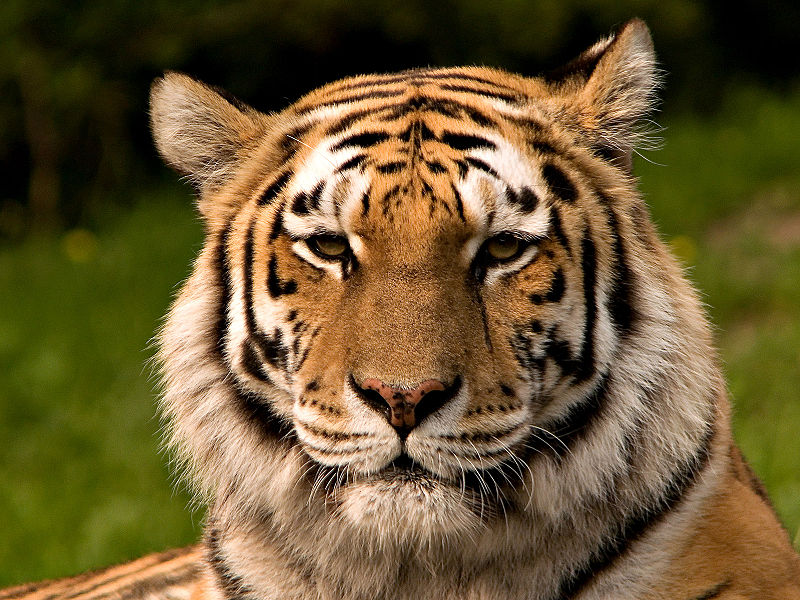
\includegraphics[width=0.5\textwidth]{tiger.jpg}}
  \caption{A picture of the same gull
           looking the other way!}
\end{figure}

\end{document}
